\documentclass[a4paper,11pt]{article}
\usepackage[T1]{fontenc}
\usepackage[utf8]{inputenc}
\usepackage{lmodern}
\usepackage{hyperref}
\usepackage{graphicx}
\usepackage{rotating}
\usepackage{listings}
\usepackage{color}
\usepackage{listings}
\usepackage{pdfpages}

\title{Advanced Algorithms - part 3 (exc 7-9)}
\author{Arash Rouhani (rarash@student.chalmers.se) - 901117-1213}

\begin{document}

\maketitle

\section{Bigamical Matching}

Recall the standard flow-solution to bipartite matching.
By making a minor edit to that, we can get it to solve for our problem.
I will first shortly recall the standard solution, then I will
clarify how our problem \emph{and} solution differs.
Lastly I will motivate why that solution solves for our modified version.

In the standard problem we have that each $X$ matches to at most $1$ $Y$.
The solution then is to create graph with a source node $s$ and
sink node $t$. Then connect edges $s \to x$ and $y \to t$. Also
we add the edges from $E$, that is $x \to y$ $(x,y) \in E$,
this time the edges are directed. All edges in this constructed graph
has capacity $1$.
If we solve for maximum flow in this graph, we will get an optimal
solution. $x$ matches to $y$ iff $f_{(x,y)} = 1$.

But the problem statement is that $X$ can match to at most $2$ $Y$.
I claim that to accomodate for this difference, the only modification
is to give capacity $2$ for the $s \to x$ edges.
We still have the exact same interpretation for $f_{(x,y)} = 1$.

Motivation: $0 \leq f_{(s, x)} \leq 2$ and $0 \leq f_{(y, t)} \leq 1$
represents number of matches $x$ and $y$ has respectively,
this matches the problem. $0 \leq f_{(x, y)} \leq 1$ is indeed
a "boolean" for if $x$ matches to $y$.

A motivating example: For a fixed
$x$, if $f_{(s, x)} = 2$, the rule of \emph{flow conservation}
forces for $x$ to match to two different $y_1$ and $y_2$.
$y_1 \neq y_2$ because that otherwise would contradictory imply
$f_{(x, y_1)} = 2 \leq 1$. Flow conservation
at all node types have a semantic in the problem desrciption.
We just looked at node type $x$. Similar simple analysis
can be done for $s$, any $y$, and $t$ nodes as well,
but we ommit that.

Since this is only a flow problem, this can be solved
in polynomial time.

\section{Dominos on a grid-set}

This is also matching! But between which two "genders"?
We will partition $Q$ into $X,Y \subseteq Q$.
If we paint the squares on $Q$ like a chess board, then we let
$X$ be the white and $Y$ be the black squares.
The intuition here is that if you put a domino brick on a chess board
it will cover one white and one black square. So if a brick covers
$q_1,q_2 \in Q$, we know that we can write it as
$x=q_1 \in X$ and $y=q_2 \in Y$.

One should now recall the problem's
constraints on brick placement, "two adjacent squares" means one
square is black the other white. "must not overlap" will mean that
we can actually see this as a matching problem, $x$ and $y$ are
matched if they share the same domino brick. In the original
marriage problem a person (male or female) can't marry twice,
here a square (black or white) can't have two domino bricks covering it.

Algorithm-wise we use maximum flow.
We construct the bipartite graph
$G = (X, Y, \{(x,y) | x \in X, y \in Y, adjacent(x, y))$
and solve the matching problem. We put a domino on square $x$ and $y$
iff $f_{(x,y)} = 1$. We have many times discussed how bipartite
matching is solved, both in class and in the previous problem.

An augmenting path can be found in
$O(E)=O(V)$ and each found path increases flow by $1$, that increment
won't be found more than $V$ times as that would "overflow".
This can run in $O(V^2)$ time.
Hopcroft-Karp algorithm for bipartite matching even gives
running time of $O(V^{1.5})$.

\section{Multi-source/sink Edge-disjoint connectivity}

We are given $G = (V, E)$, we have some sources $s_1,..,s_k \in V$
and sinks $t_1,..,t_k \in V$. We solve the problem with maximum
flow by contructing a flow-graph $G'$ from $G$. We then contsruct the
paths by "following flows".
Lets now look at it a bit more in detail.

Construct the graph $G' = (V \cup \{S, T\}, E \cup E')$.
So $S$ and $T$ are new nodes, the \emph{real} source and sink.
$S$ will provide $s_1..s_k$ with flow.
Looking at $G$, the small sources will have their own
production, while in reality it comes from $S$. $T$ will
in the same sense be a supersink for $t_1..t_k$.
For $S$ and $T$ to really be what I just described we
set $E' = \{(S, s_i) | i=1..k\} \cup \{(t_i, T) | i=1..k\}$.
We set that all edges have the capacity $1$.

The maximum flow $m$ from this network will be the number
of paths we can construct. If $m=k$ then we indeed can
find $k$ paths from $s_i$ to $t_j$.
If $m \neq k$ then there is no solution to the problem.
If $m=k$ we try to find the actual $k$ paths.
Below we give an algorithm for finding the paths given the
flow. But first we introduce our auxiliary graph search GS.

\textbf{GS: }
GS is a graph search like DFS or BFS. It is a edge-traversing
function that doesn't care what nodes it has visited.
In only maintains which current node it is and and will
continue traversing an edge until it reaches its given goal-node $T$.
It starts from a node $S$.
We must guarantee it always have an edge to take until it
reaches $T$.
\textbf{End.}

\textbf{Algorithm: }
GS in the directed graph $G'$ from $S$ until $T$.
Use only edges where
$f_e=1$ and consume ($f_e:=0$) that flow when traversing on it.
Add the \emph{trimmed} path to the list of paths,
trimmed means $S$ and $T$ are removed from the path's
front and rear respectively.
Do the GS $k$ times.
\textbf{End.}

Correctness: We must show that the trimmed path actually is from
a $s_i$ to a $t_j$ and they are unique for each path.
Also we must show that the algorithm terminates and we actually
will find a path to $T$.

A path from $S$ to $T$
will when trimmed be from some $s_i$ and some $t_j$
as of the construction of $G'$.
Furthermore since we consume the particular edges
$(S, s_i)$ and $(t_j, T)$, the next GS must find
different $s$ and $t$ nodes.

Will we run GS $k$ times succesfuly when we have a max flow of $k$?
First observe that GS will always have an edge to take (will never get stuck).
This follows from that all nodes
but $S$ and $T$ \emph{conserves flow}, if you can enter
the node you can leave it as well. This observation also leads to
that there will be $k$ paths:
Once starting searching from $S$, there will the first $k$ times
be a first node $s_i$ to visit since outflow from $S$ was $k$.
And if we can enter $s_i$ we must then able to leave to another
node, and this will go on until we visit $T$.

Finally as for termination. All capacities are $1$ and the
edges are finite, therefor this will terminate as each used edge
consumes one flow which would vanish if the graphsearch would
never terminate.

Ok, this was our motivation for the algorithm correctness and we are done.

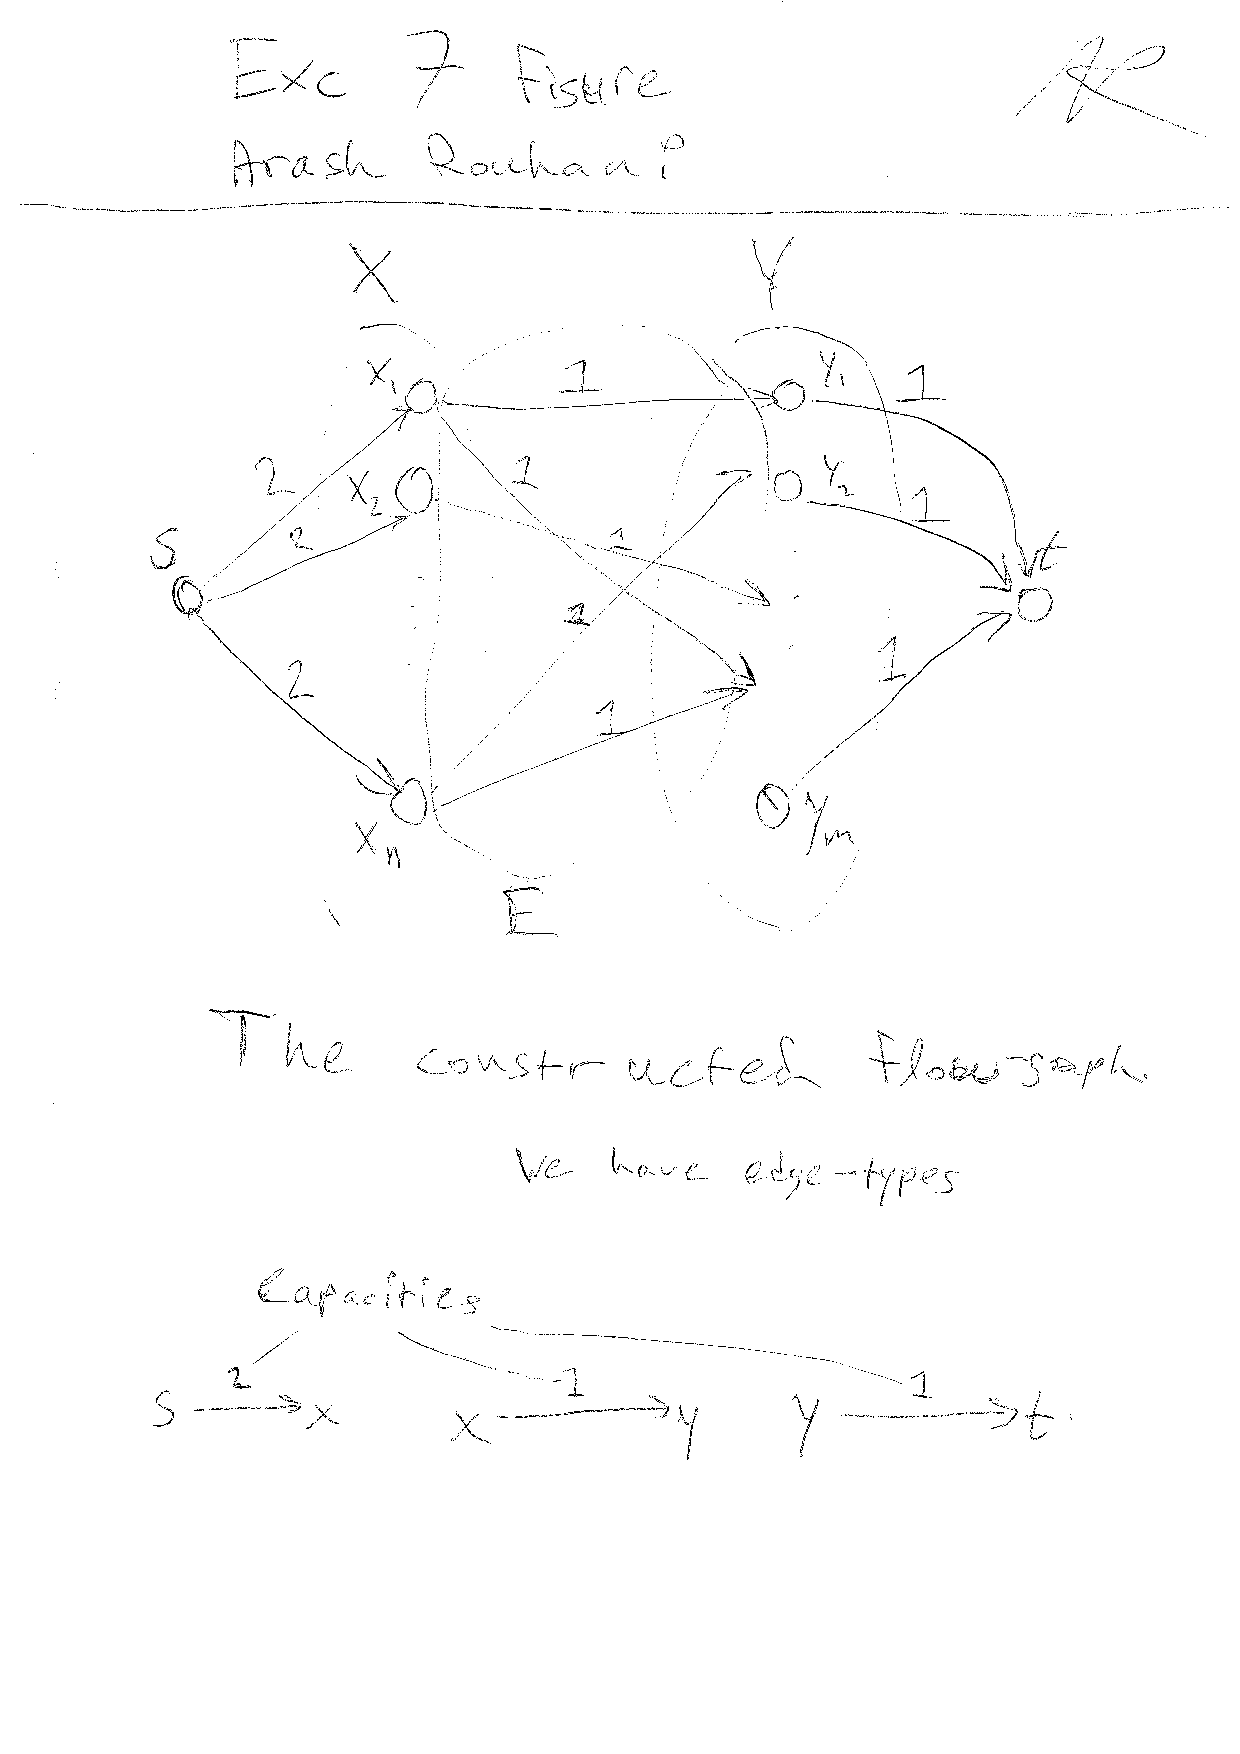
\includepdf[pages=1-3]{20111116161943449.pdf} % probably needed later

\end{document}
